\chapter{Analyse}

\section{Integrationsansätze - Industrie 4.0}
\subsection{Konsolidierung der Netzwerkkommunikation}

TODO - siehe Testsystem Martin - alles spricht OPC UA

\subsection{TODO - Gateways zum Übersetzen der Kommunikation}

TODO - siehe Trumpf, axoom -> Gateways übersetzen von heterogener Netzwerkkommunikation in Protokollstandard für unternehmensübergreifende bzw. externe Kommunikation.
Ansatz: Softwareschwachstellen, Softwarefehler, müssen viele Herstellerprotokolle unterstützen - Probleme?

\subsubsection{Security-Komponenten}
\subsubsection{Router}
\subsubsection{Gateways}

\section{Protokollstandards}
\subsection{OPC UA}
\subsection{MConnect}
\subsection{M2M-Kommunikation}
TODO - Maschine 2 Mensch und Maschine 2 Maschine -> M2M Protokolle
\subsection{TODO}

\section{Sicherheitsanforderungen des Kommunikationsstacks}
\subsection{Physical Layer}
\subsection{Data Link Layer}
\subsection{Network Layer}
\subsection{Transport Layer und End2End Security}
\subsection{Prozess- und Businesslogik - Application Layer}

\section{Probleme bei Migration alter Systeme}
\subsection{Inkompatibilität}
\subsection{spezielle bzw. proprietäre Protokolle}
\subsection{besondere Anforderungen der Shop-Floor-Ebene}

\section{Angriffsvektoren}
\subsection{Verschlüsselung}
\subsection{Paketversand}
\subsection{TODO}

\section{Auswertung der Ergebnisse}

\section{Maßnahmenkatalog}
\subsubsection{Defense in Depth Strategie - TODO (Kuipers,2006)}

TODO - Beschreibung und Einordnung der Defense in Depth Strategie

\begin{figure}[h]
    \centering
    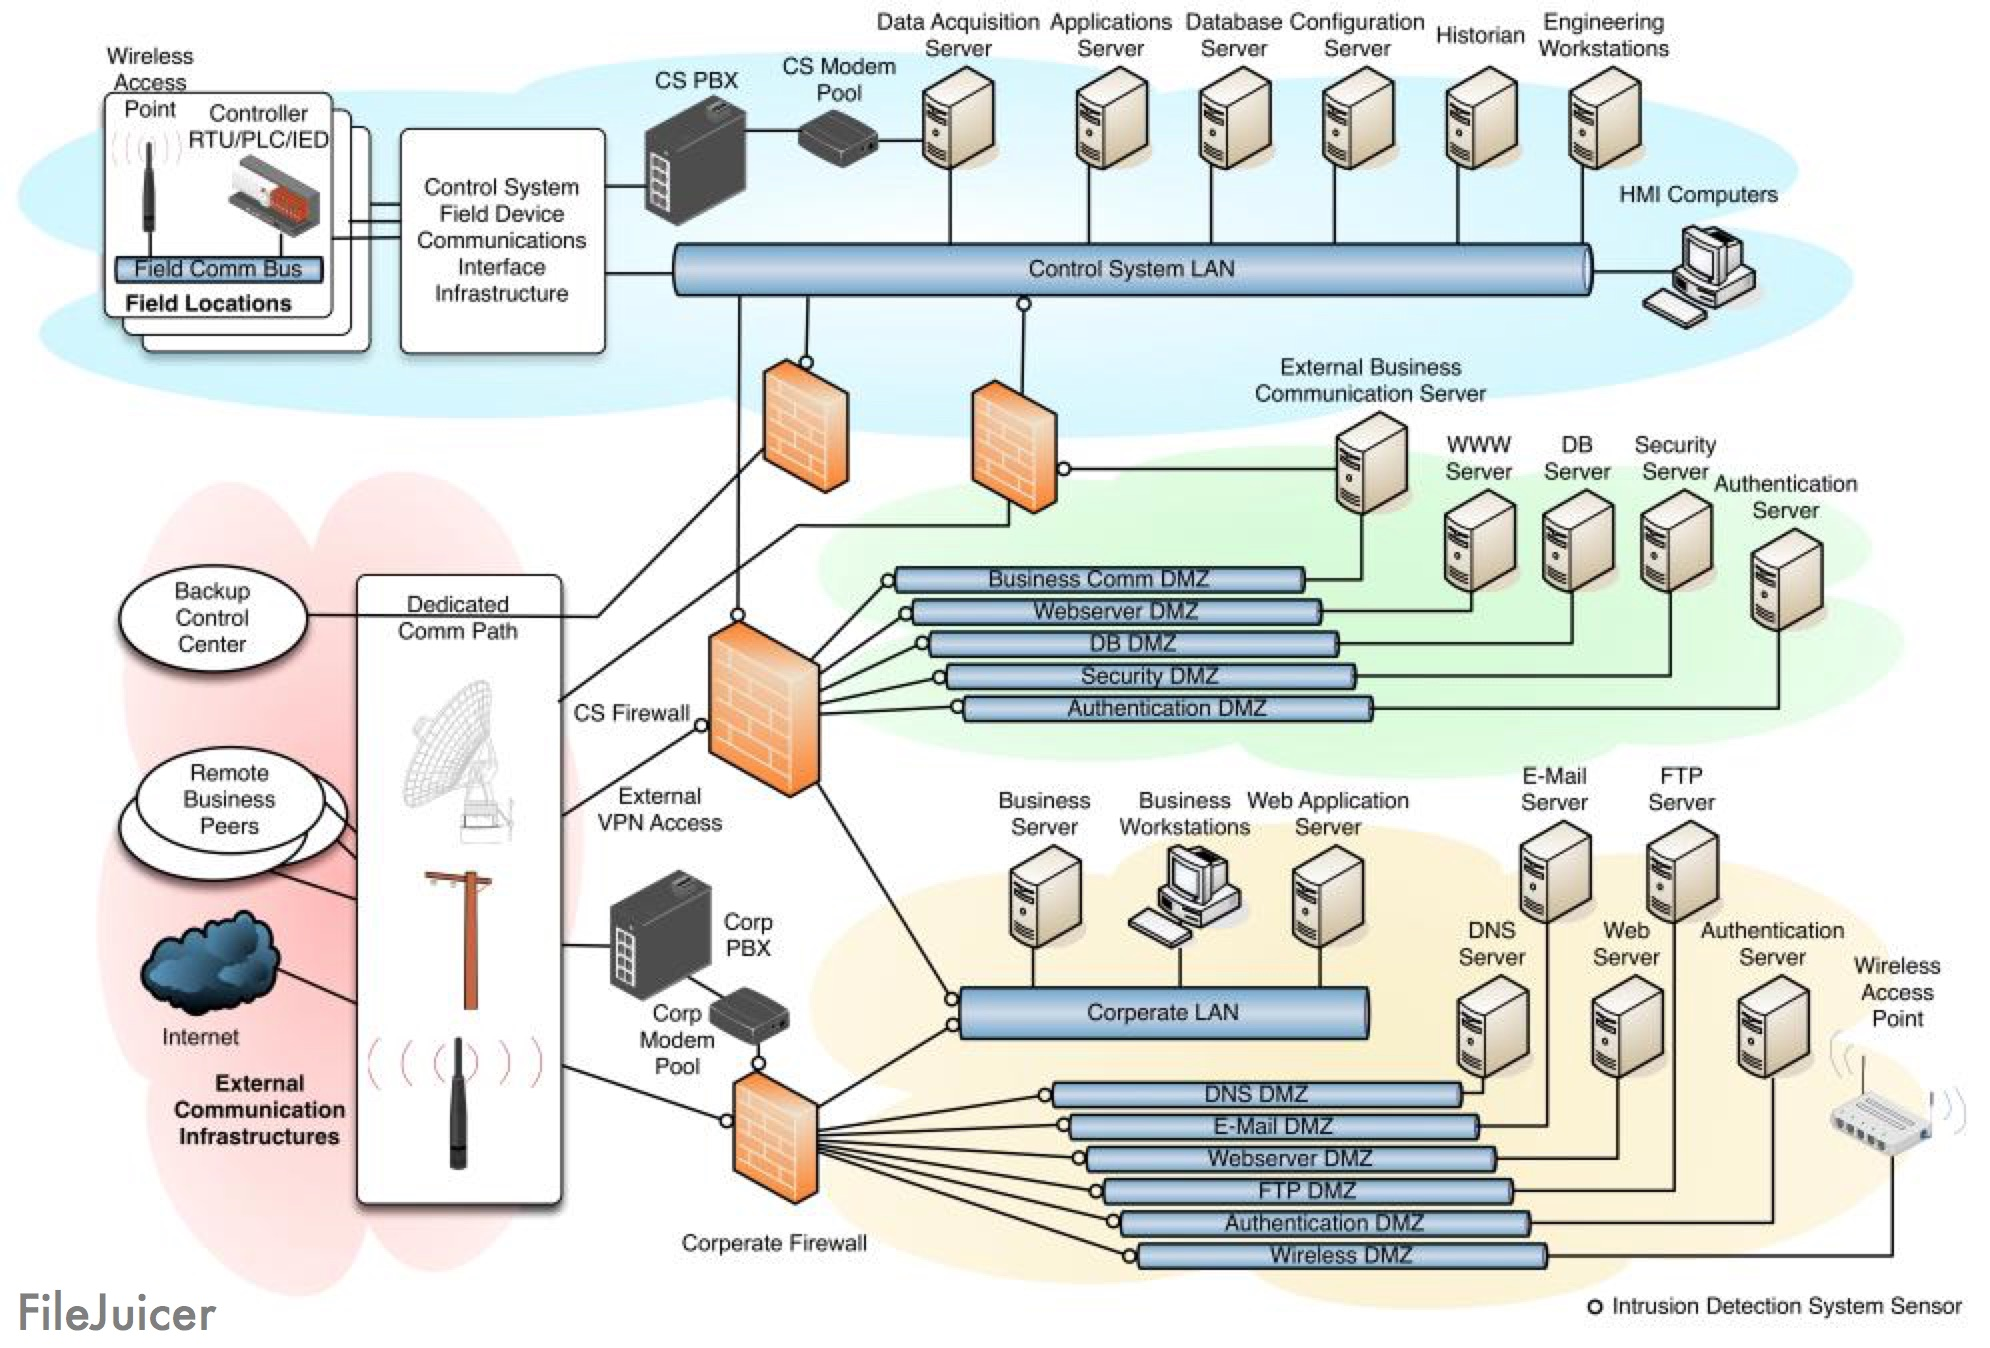
\includegraphics[width=15cm]{defense-in-depth-strategie}
    \caption{Defense in Depth Strategie - TODO ref. Kuipers,2006}
    \label{Kap3:Defense-in-Depth}
\end{figure}

